% Standard 10pt
\documentclass[a4paper,twoside, openright]{report}

\usepackage[utf8]{inputenc}
\usepackage{fontspec, emptypage}
\usepackage[a4paper, left=2.5cm, right=2.5cm, bottom=2.8cm, top=2.8cm]{geometry}
\usepackage[ngerman,english]{babel}
\usepackage{fancyhdr, graphicx, amsmath, hyperref, longtable, float, enumitem, blindtext}
% For Bibliography
\usepackage{natbib}
\bibliographystyle{authordate1}
% For Abkürzungsverzeichnis
\usepackage{acronym}
% For appendix
\usepackage[toc,page]{appendix}
% For tikz
\usepackage{calc, ifthen, tikz}
% For including pdfs
\usepackage{pdfpages}
% Caption setup
\usepackage[tableposition=b]{caption}
\captionsetup[longtable]{skip=1em}
% Important for longtable
\usepackage{arydshln}

\hypersetup{
	colorlinks,
	citecolor=black,
	filecolor=black,
	linkcolor=black,
	urlcolor=black
}

\renewcommand{\baselinestretch}{1.2}
\newcommand{\tabitem}{~~\llap{\textbullet}~~}
\newcommand{\HRule}{\rule{\linewidth}{0.3mm}} % Defines a new command for the horizontal lines, change thickness here

\addto\captionsngerman{\let\appendixtocname\appendixname%
	\let\appendixpagename\appendixname}

\title{Bachelor Thesis}

\parindent 0pt

\begin{document}

% ----------------------------------------
% Titelblatt
% ----------------------------------------
\begin{titlepage}
\begingroup
\centering
\vspace*{\baselineskip}

\thispagestyle{empty}

\begin{figure}[H]
	\centering
	\begin{minipage}{.49\textwidth}
		\centering
		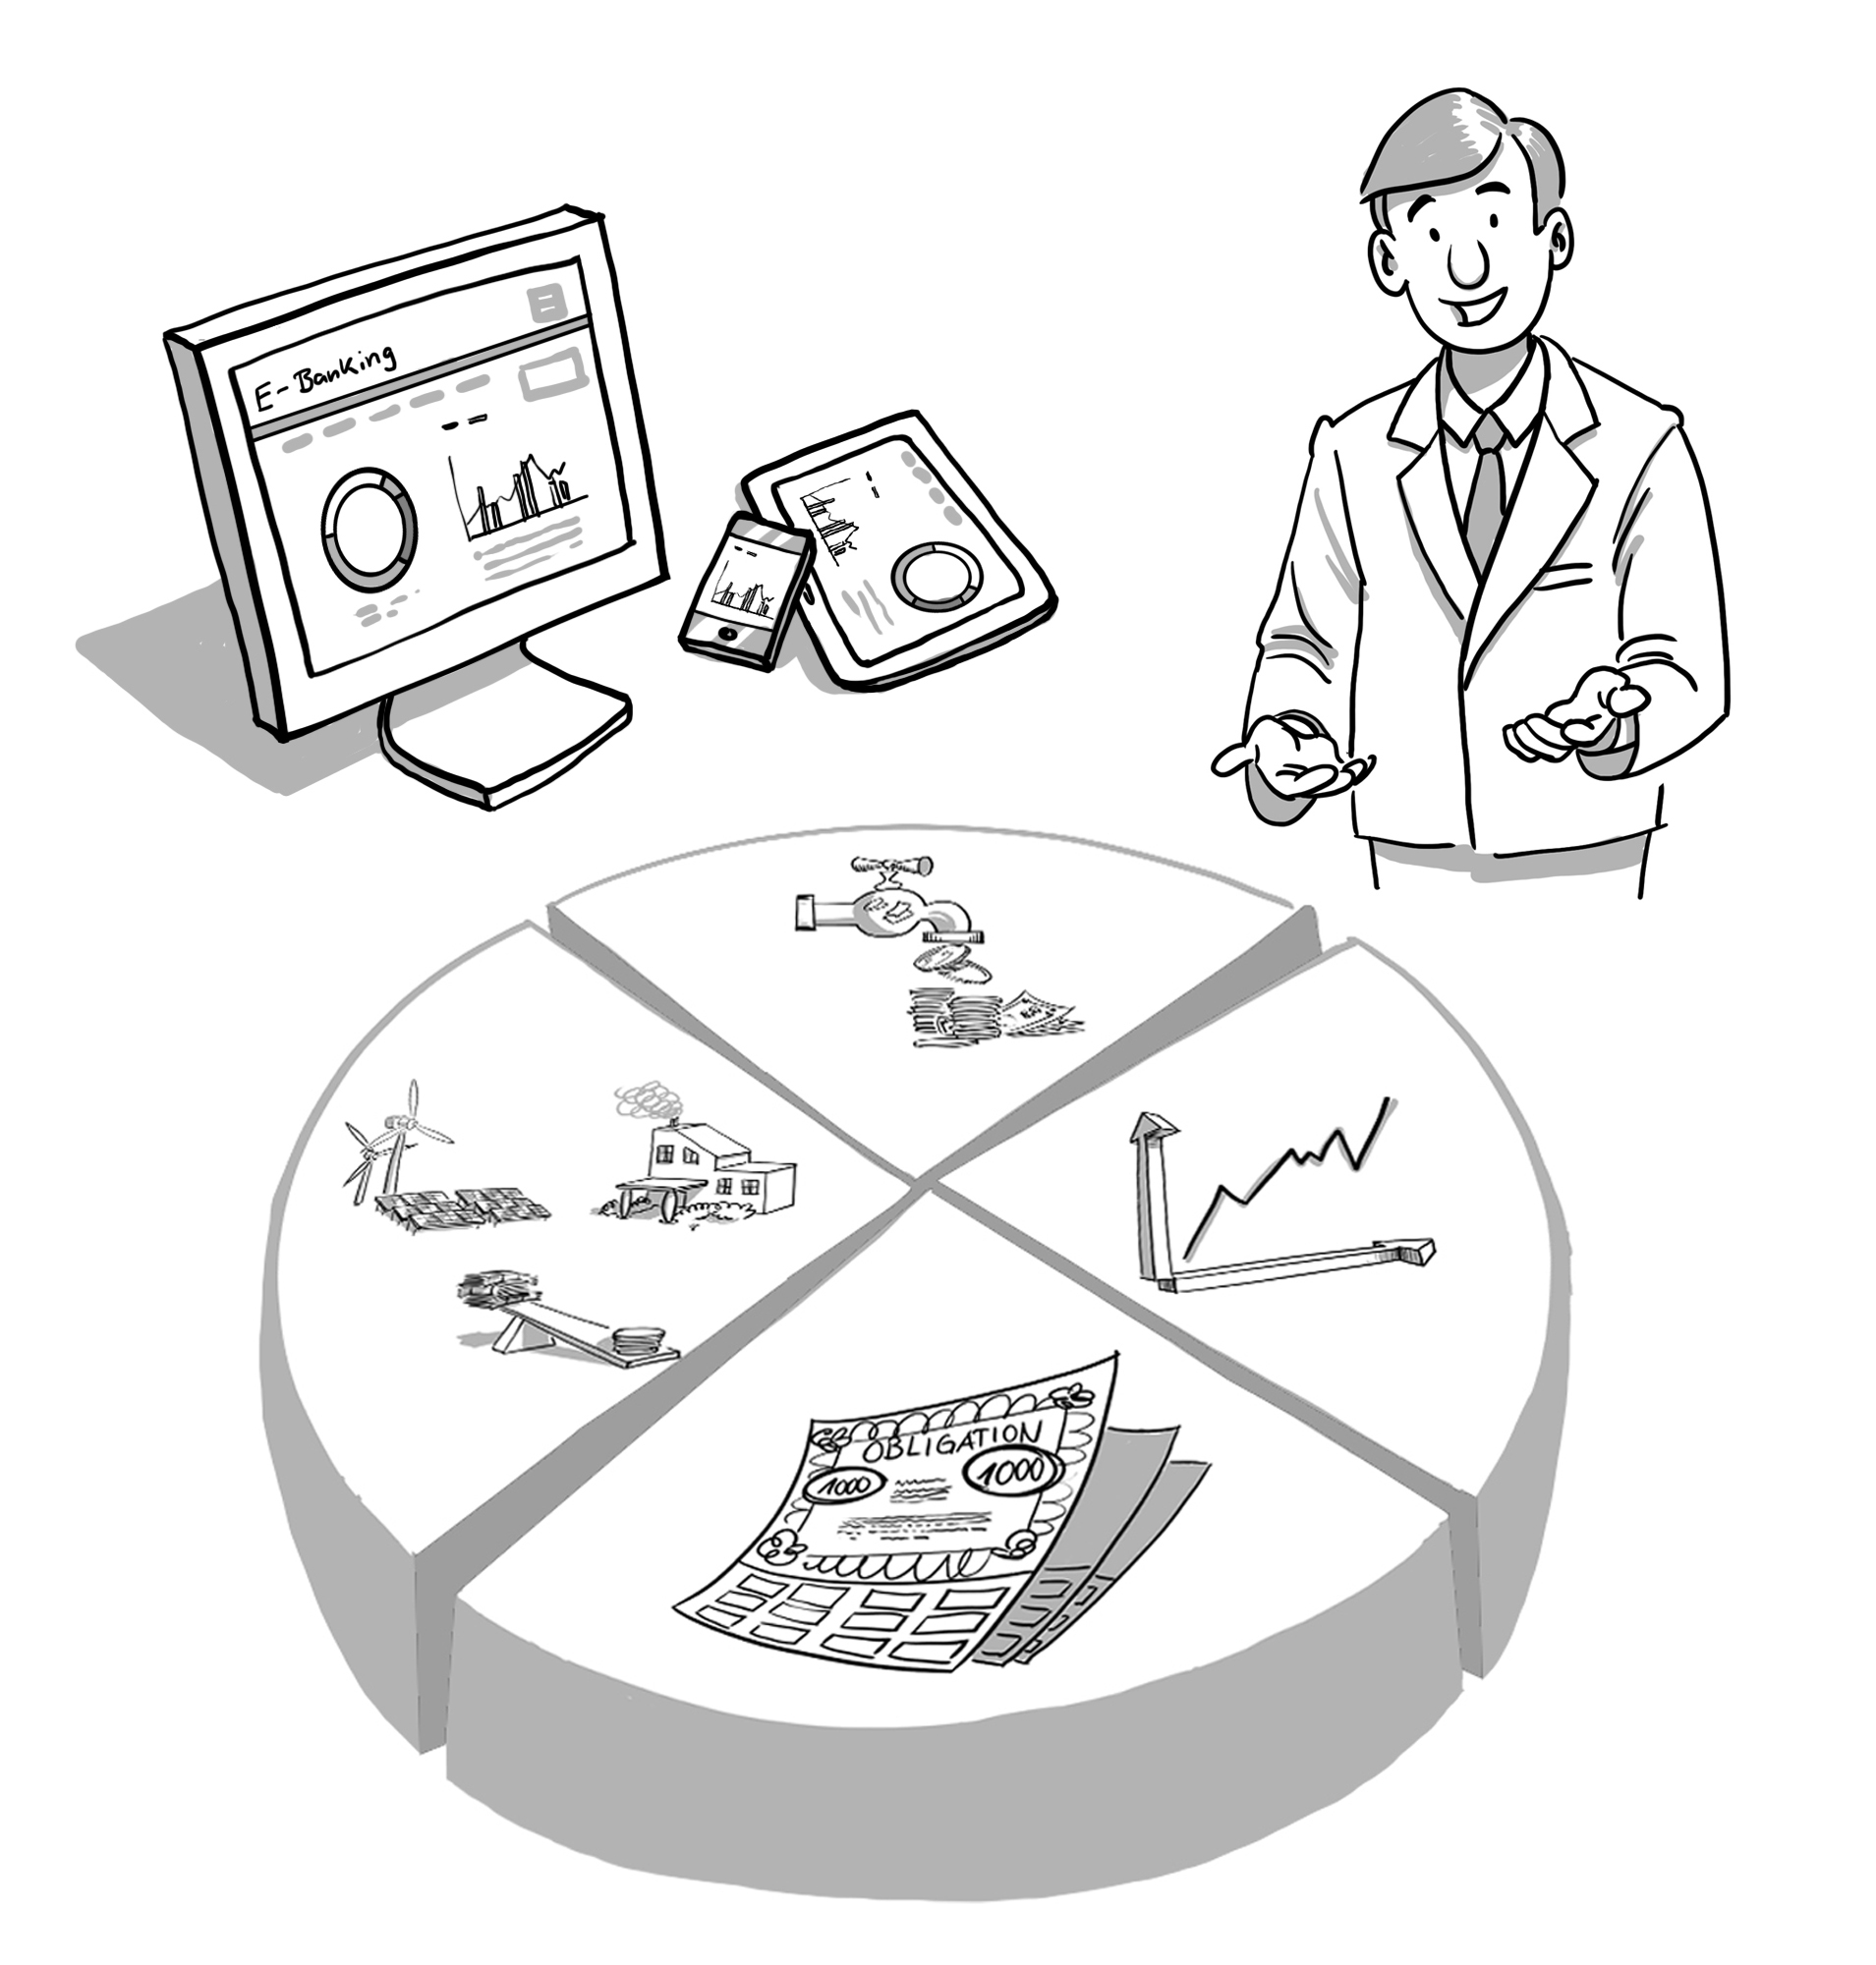
\includegraphics[scale=0.3]{img/InvestmentSolutions.jpg}
	\end{minipage}
\end{figure}

\vspace*{1\baselineskip}

\HRule \\[0.4cm]
{\LARGE \textbf{Entwicklung einer tabletbasierten Applikation zur Unterstützung der Arbeitspraktiken in der Hypothekarberatung}}
\HRule \\[1.5cm]

\vspace*{1\baselineskip}

{\large \textbf{Bachelor Thesis}}

\vspace*{1\baselineskip}

\scshape % Small caps
\large University of Zurich - Institut für Informatik \\ \vspace{3.5mm}
\large Information Management Research Group \\ \vspace{3.5mm}
\large Prof. Dr. Gerhard Schwabe

\vspace*{0.5\baselineskip}



\begin{align*}
\textbf{Verfasser:} &\ \text{Pascal Zehnder} \\
&\ \text{13-712-336} \\
&\ \text{pascal.zehnder@bf.uzh.ch} \\
\textbf{Geburtsort:} &\ \text{Schwyz} \\
\textbf{Studienrichtung:} &\ \text{Wirtschaftsinformatik} \\
\textbf{Betreuender Assistent:} &\ \text{Mehmet Kilic} \\
\textbf{Zweitbetreuer:} &\ \text{Mateusz Dolata} \\
\textbf{Abgabe der Arbeit:} &\ \text{19.04.2017} \\
\end{align*}

\endgroup
\end{titlepage}

\newpage

\pagenumbering{roman}

% ----------------------------------------
% Abstract auf English
% ----------------------------------------
\selectlanguage{english}%
\chapter*{Abstract}
In numerous industries modern technologies more and more find its application. Multiple surveys about advisory servies in the financial sector came to the conclusion that various banking institutions are still using pen and paper during an advisory service. IT-supported artefacts furthermore can't find their application in financial advisory services.\\

In previous works a fundamental acceptance of using IT-supported artefacts in financial advisory services could be recognized on the part of customer and advisor. In comparison to a conventional advisory service an additional benefit could be recognized.\\

Based on the analysis of a previous prototype and particular conventional advice giving, as well as interviews with customers and advisors, requirements for an optimally designed prototype were generated. The main focus of the task was on the development of the prototype. The implemented prototype was then evaluated in a focus group. The feedback of the participants confirmed the improvement of the usability and labor practices of the advisors which was a consequence of conscious adjustments and newly developed features.

% ----------------------------------------
% Inhaltsübersicht
% ----------------------------------------
\tableofcontents

\newpage

% ----------------------------------------
% Start des eigentlichen Inhalts
% ----------------------------------------
\pagestyle{headings}
\pagenumbering{arabic}
\section{Introduction}

\newpage

% ----------------------------------------
% Literaturverzeichnis
% ----------------------------------------
\selectlanguage{ngerman}
\bibliography{bachelor_thesis}


\end{document}
